\begin{figure}[htbp]
  \centering
  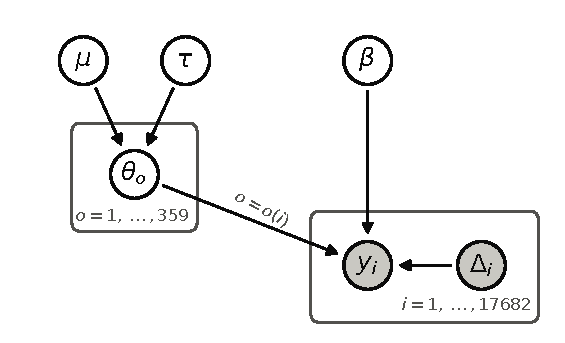
\includegraphics[width=\linewidth]{model.pdf}
  \caption{The model as a Bayesian network. Shaded nodes are observed and white nodes are unknown; plates repeat their content for each of the 359 openings and the 17,682 decisive games. Game $i$ is played in opening $o(i)$; its result is $y_i = 1$ if White wins and $0$ if Black wins, and $\Delta_i$ is the rating of White minus the rating of Black, divided by 400. $y_i \sim \text{Bernoulli}(\operatorname{logit}^{-1}(\theta_{o(i)} + \beta \Delta_i))$, $\theta_o \sim \mathcal{N}(\mu, 1/\tau)$, $\mu \sim \mathcal{N}(0, 0.5^2)$, $\beta \sim \mathcal{N}(\log 10, 1^2)$ and $\tau \sim \text{Gamma}(1, 0.05)$ (shape and rate); we report $\sigma = 1/\sqrt{\tau}$.}
  \label{fig:model}
\end{figure}
